\section{The pinned bounds and the right angle}\label{sec:right-angle}

Baek shows that a balanced maximum sofa $S_\omega$ with $\abs{S_\omega}\ge11/5$ and rotation angle $\omega\in[\omega_0,\pi/2)$
has a rotated copy that turns through the full right angle \baek{Thm.~1.5.2}. The proof uses the balance only
through two inequalities, $w^\circ_K\le\sigma_K(\pi/2)$ and $z^\circ_K\le\sigma_K(\omega)$, which bound the wedge gaps on the two floors $y=0$ and $l(\omega,0)$ by the lengths of the sides of the
cap on the opposite walls $y=1$ and $l(\omega,1)$ \baek{Thm.~4.1.4}. We
prove these inequalities for $K_*$ from the defect bounds of \cref{sec:variations}, and then follow
Baek's proof with them as hypotheses. In \cref{sec:pinned-bounds,sec:triangle} we have $\omega<\pi/2$, and $K_*$ is as in \cref{sec:selection};
\cref{prop:U} also covers $\omega=\pi/2$.

\subsection{The pinned bounds}\label{sec:pinned-bounds}

For a cap $K\in\Kc_\omega$ and $t\in(0,\omega)$ let
\[
  w_K(t)=h_K(0)-\frac{h_K(t)-1}{\cos t},\qquad
  z_K(t)=h_K(\omega+\tfrac\pi2)-\frac{h_K(t+\pi/2)-1}{\cos(\omega-t)},
\]
the \emph{wedge gaps}: with $A=(h_K(0),0)=A_K^-(0)$ and $C=h_K(\omega+\pi/2)v_\omega=C_K^+(\omega)$ the ends of the
upper boundary of $K$ (see \eqref{eq:ends}), $w_K(t)$ is the distance from $A$ to the point
$W_K(t)=((h_K(t)-1)/\cos t,0)$ where the inner wall $b_K(t)$ meets the $x$-axis, and $z_K(t)$ is the
distance from $C$ to the point where $d_K(t)$ meets $l(\omega,0)$ \baek{Def.~2.5.5}. Let
$w^\circ_K=\inf_{t\in(0,\omega)}w_K(t)$ and $z^\circ_K=\inf_{t\in(0,\omega)}z_K(t)$ \baek{Def.~4.1.1}.
As $t\to\omega$, $w_K(t)\to h_K(0)$, so $w^\circ_K\le h_K(0)$; as $t\to0$, $z_K(t)\to h_K(\omega+\pi/2)$, so $z^\circ_K\le h_K(\omega+\pi/2)$.

\begin{lemma}[wedge gaps and the polyline]\label{lem:wedge}
Every polygon cap $K\in\Kc_\Theta$ satisfies $w^\circ_K\le\tau_K(\pi/2)$ and $z^\circ_K\le\tau_K(\omega)$.
\end{lemma}

This is the first half of the proof of \baek{Thm.~4.1.2}.

\begin{proof}
The bottom edge $e_K(3\pi/2)=K\cap\{y=0\}$ is the segment from $O$ to $A=(h_K(0),0)$, so
$\sigma_K(3\pi/2)=h_K(0)$. A point $(x,0)$ of $\cN_\Theta(K)$ lies in $F_\omega$, so $x\ge0$, and in some
$Q^-_K(t)$, $t\in\Theta$, so $x\cos t<h_K(t)-1$, that is $x<h_K(0)-w_K(t)\le h_K(0)-w_K^\circ$. Hence
$\cN_\Theta(K)\cap\{y=0\}\subset[0,h_K(0)-w^\circ_K)\times\{0\}$, and by \cref{fact:sides}\ref{fact:sides:floor}
\begin{align*}
  h_K(0)-\tau_K(\pi/2)&=\sigma_K(3\pi/2)-\tau_K(\pi/2)\\
  &=\Hone\bigl(\cN_\Theta(K)\cap l(\pi/2,0)\bigr)\le h_K(0)-w^\circ_K,
\end{align*}
where we used $w^\circ_K\le h_K(0)$. The second inequality is the same argument on the line $l(\omega,0)$, with
the bottom edge $e_K(\omega+\pi)=[O,C]$ of length $\sigma_K(\omega+\pi)=h_K(\omega+\pi/2)$, the points
$\lambda v_\omega$ of $Q^-_K(t)$, which have $\lambda<h_K(\omega+\pi/2)-z_K(t)$, and
\cref{fact:sides}\ref{fact:sides:floor} with $t=\omega$.
\end{proof}

\begin{lemma}[continuity]\label{lem:cont}
For caps $K,K'\in\Kc_\omega$ with $\dH(K,K')=\eps$, $\abs{w^\circ_K-w^\circ_{K'}}\le(1+\sec\omega)\eps$ and
$\abs{z^\circ_K-z^\circ_{K'}}\le(1+\sec\omega)\eps$.
\end{lemma}

\begin{proof}
For $t\in(0,\omega)$, $\abs{w_K(t)-w_{K'}(t)}\le\eps+\eps\sec t\le(1+\sec\omega)\eps$; similarly for $z$, since
$\cos(\omega-t)\ge\cos\omega$. The infima differ by at most as much. \baek{Lemma~4.1.1}
\end{proof}

Baek obtains \baek{Thm.~4.1.4} from the weak convergence of surface area measures \baek{Thm.~4.1.3} and the Portmanteau theorem. The following elementary
lemma, which uses only support functions, replaces that step.

\begin{lemma}[upper semicontinuity of edge lengths]\label{lem:usc}
If convex bodies $K_j\to K$ in $\dH$, then $\limsup_j\sigma_{K_j}(t)\le\sigma_K(t)$ for every $t$.
\end{lemma}

\begin{proof}
For $0<\delta<\pi$,
\begin{align*}
  h_K(t+\delta)&\ge\ip{v_K^+(t)}{u_{t+\delta}}=h_K(t)\cos\delta+\ip{v_K^+(t)}{v_t}\sin\delta,\\
  h_K(t-\delta)&\ge\ip{v_K^-(t)}{u_{t-\delta}}=h_K(t)\cos\delta-\ip{v_K^-(t)}{v_t}\sin\delta.
\end{align*}
Adding, and using $\sigma_K(t)=\ip{v_K^+(t)-v_K^-(t)}{v_t}$,
\[
  \sigma_K(t)\le\Delta_K(\delta)=\frac{h_K(t+\delta)+h_K(t-\delta)-2h_K(t)\cos\delta}{\sin\delta}.
\]
$\Delta_K(\delta)$ depends continuously on the values of $h_K$, so $\Delta_{K_j}(\delta)\to\Delta_K(\delta)$ and
$\limsup_j\sigma_{K_j}(t)\le\Delta_K(\delta)$ for every $\delta$. By \cref{fact:convex}\ref{fact:convex:vertices},
$\Delta_K(\delta)\to\ip{v_K^+(t)-v_K^-(t)}{v_t}=\sigma_K(t)$ as $\delta\downarrow0$.
\end{proof}

\begin{proposition}[pinned bounds]\label{prop:pinned-bounds}
$w^\circ_{K_*}\le\sigma_{K_*}(\pi/2)$ and $z^\circ_{K_*}\le\sigma_{K_*}(\omega)$.
\end{proposition}

\begin{proof}
Take the selection $K_j\to K_*$ of \cref{prop:selection} in $[-R_0,R_0]\times[0,1]\subset\{\norm p\le R\}$,
$R=R_0+1$, and $\eta_j=\dH(K_j,K_*)\to0$; at every sampled normal $\abs{h_{K_j}-h_*}\le\eta_j$, and the total
weight is $\bar\nu<1$. By \cref{cor:twosided} at $t=\pi/2$, with $e_j=(2+4\gamma_\omega)\eta_j$,
$\abs{\sigma_{K_j}(\pi/2)-\tau_{K_j}(\pi/2)}\le e_j$; so by \cref{lem:wedge}
\[
  w^\circ_{K_j}-e_j\le\tau_{K_j}(\pi/2)-e_j\le\sigma_{K_j}(\pi/2).
\]
By \cref{lem:cont}, $w^\circ_{K_j}\to w^\circ_{K_*}$, and by \cref{lem:usc},
$\limsup_j\sigma_{K_j}(\pi/2)\le\sigma_{K_*}(\pi/2)$. This gives the first inequality. For the second use
$t=\omega$, where \cref{cor:twosided} divides by $\sin\omega>0$.
\end{proof}

\subsection{The triangle in the niche}\label{sec:triangle}

Let $\omega\in[\omega_0,\pi/2)$, so that $\omega>\pi/4$. Put $c=c_\omega=\sec\omega-\tan\omega$, so that
$o_\omega-v_0=c\,u_0$ and $o_\omega-u_\omega=c\,v_\omega$ \baek{Prop.~4.2.1}, and let $\Delta_\omega$ be the
triangle with vertices $O$, $cu_0$, $cv_\omega$, which cuts off the corner $O$ of $P_\omega$. Let
$d_{\min}=5/4$ if $\omega<\tan^{-1}(11/5)$ and $d_{\min}=11/10$ otherwise, and for $d\in[0,\tan\omega]$ let
$R_{\omega,d}=P_\omega\cap H_-(0,d+c)\cap H_-(\omega+\pi/2,d+c)$ be $P_\omega$ without its two acute corners.

\begin{fact}[numerical inequalities at the corner]\label{fact:corner}
Let $\omega\in[\omega_0,\pi/2)$.
\begin{enumerate}[label=(\alph*)]
\item $\abs{R_{\omega,d_{\min}}}<11/5$. \baek{Lemma~4.2.2}
\item If $d\in[d_{\min},\tan\omega]$, $r_y=1-d\cot\omega\ge0$ and $g=\sqrt{1-r_y^2}$, then $d\sin\omega>1$ and $g>2\cos\omega$.
\baek{Lemma~4.2.4, in the range $[\sec^{-1}(2.2),\pi/2)$ of its proof and of its use (E9)}
\end{enumerate}
\end{fact}

\begin{lemma}[the triangle lies in the niche]\label{lem:triangle}
Let $\omega\in[\omega_0,\pi/2)$ and $K\in\Kc_\omega$ with $\cA_\omega(K)\ge11/5$, $w^\circ_K\le\sigma_K(\pi/2)$ and
$z^\circ_K\le\sigma_K(\omega)$. Then for some $t_\sharp\in(0,\omega)$ the three vertices $O$, $cu_0$, $cv_\omega$ of
$\Delta_\omega$ lie in $Q^-_K(t_\sharp)$.
\end{lemma}

This is \baek{Thm.~4.2.5} for a cap that satisfies the pinned bounds, in place of a balanced maximum cap; the
proof there uses balance only through them.

\begin{proof}
\emph{Step 1: a long cap.} Since $\abs K\ge\cA_\omega(K)\ge11/5>\abs{R_{\omega,d_{\min}}}$ and $K\subset P_\omega$,
$K$ is not contained in $R_{\omega,d_{\min}}$, so $h_K(0)\ge d_{\min}+c$ or $h_K(\omega+\pi/2)\ge d_{\min}+c$.
We may assume the first. Otherwise replace $K$ by its mirror image $K^{\mir}$: it is a cap with the same sofa
area, and $h_{K^{\mir}}(0)=h_K(\omega+\pi/2)$, $w^\circ_{K^{\mir}}=z^\circ_K$, $\sigma_{K^{\mir}}(\pi/2)=\sigma_K(\omega)$,
so it satisfies the hypotheses; and since $M_\omega$ fixes $O$, exchanges $cu_0$ and $cv_\omega$ and maps
$Q^-_{K^{\mir}}(t)$ to $Q^-_K(\omega-t)$ \baek{Prop.~2.5.4}, the conclusion for $K^{\mir}$ at $t_\sharp$ is the conclusion
for $K$ at $\omega-t_\sharp$. Put $d=h_K(0)-c\ge d_{\min}$ and $q_0=(h_K(0),0)=A^-_K(0)\in K$. Since $K\subset P_\omega$,
$h_K(0)\le\sec\omega$, so $d\le\tan\omega$, and $q_0=(o_\omega-v_0)+d\,u_0$.

\emph{Step 2: the bottom side.} The lines $l_K(0)$ and $l_K(\omega)=l(\omega,1)$ meet at $r=(h_K(0),r_y)$ with
$r_y=1-d\cot\omega\ge0$ (as $q_0\in P_\omega$). Let $g=\sqrt{1-r_y^2}$ and $s=q_0-g\,u_0$: the triangle
$s,q_0,r$ has a right angle at $q_0$, and $\norm{r-s}=1$. For $t\in(0,\omega)$, $u_t$ is a nonnegative
combination of $u_0$ and $u_\omega$, and $K\subset H_K(0)\cap H_K(\omega)$, so $h_K(t)\le\ip r{u_t}$, and
\[
  h_K(t)-1\le\ip r{u_t}-\ip{r-s}{u_t}=\ip s{u_t}.
\]
So $s$ lies on or to the right of $W_K(t)$, that is $w_K(t)\ge g$. Hence $g\le w^\circ_K$.

\emph{Step 3: the top side.} By hypothesis, $g\le w^\circ_K\le\sigma_K(\pi/2)$. The point $o_\omega$ lies in $K$,
and it is the right end of the top edge $e_K(\pi/2)=K\cap\{y=1\}$, because $K\subset P_\omega$. So
$q_1=o_\omega-g\,u_0$ lies on $e_K(\pi/2)$, and $q_1\in K$.

\emph{Step 4: the hallway of angle $t_\sharp=\pi/2-\omega$.} Note $t_\sharp\in(0,\pi/4)\subset(0,\omega)$. Let $X=\{q_0,q_1\}\subset K$;
then $h_X\le h_K$, so $Q^-_X(t_\sharp)\subset Q^-_K(t_\sharp)$. We have $q_1-q_0=v_0-(d+g)u_0=-\alpha u_{t_\sharp}+\beta v_{t_\sharp}$ with
$\alpha=(d+g)\cos t_\sharp-\sin t_\sharp\ge0$ and $\beta=\cos t_\sharp+(d+g)\sin t_\sharp\ge0$, since $d+g\ge1>\tan t_\sharp$. So
$q_0$ maximizes $\ip\cdot{u_{t_\sharp}}$ and $q_1$ maximizes $\ip\cdot{v_{t_\sharp}}$ on $X$, and
\begin{align*}
  Q^-_X(t_\sharp)&=\{p:\ \ip p{u_{t_\sharp}}<m_1,\ \ip p{v_{t_\sharp}}<m_2\},\\
  m_1&=\ip{q_0}{u_{t_\sharp}}-1,\quad m_2=\ip{q_1}{v_{t_\sharp}}-1 .
\end{align*}

\emph{Step 5: the vertices.} By \cref{fact:corner}(b), $d\sin\omega>1$ and $g>2\cos\omega$. Now
$\ip{q_0-cu_0}{u_{t_\sharp}}=d\sin\omega>1$, so $m_1>c\cos t_\sharp>0$; and
$\ip{q_1-cv_\omega}{v_{t_\sharp}}=\ip{u_\omega-gu_0}{v_{t_\sharp}}=-\cos2\omega+g\cos\omega>1$ (this is
$g>2\cos\omega$, as $1+\cos2\omega=2\cos^2\omega$), so $m_2>c\cos(\omega-t_\sharp)>0$. Then $O$ satisfies both
inequalities. For $cu_0$: $\ip{cu_0}{u_{t_\sharp}}=c\cos t_\sharp<m_1$ and $\ip{cu_0}{v_{t_\sharp}}=-c\sin t_\sharp<0<m_2$. For $cv_\omega$:
$\ip{cv_\omega}{u_{t_\sharp}}=-c\sin(\omega-t_\sharp)<0<m_1$ and $\ip{cv_\omega}{v_{t_\sharp}}=c\cos(\omega-t_\sharp)<m_2$. So the
three points lie in $Q^-_X(t_\sharp)\subset Q^-_K(t_\sharp)$.
\end{proof}

\subsection{A rotated copy turns through the right angle}

\begin{lemma}[the width of the sofa]\label{lem:width}
Let $\omega\in(0,\pi/2)$ and $K\in\Kc_\omega$, and suppose that $O,cu_0,cv_\omega\in Q^-_K(t_\sharp)$ for some
$t_\sharp\in(0,\omega)$. Then
\begin{enumerate}[label=(\alph*)]
\item every point $\lambda u_0+\mu v_\omega$ with $\lambda,\mu\ge0$ and $\lambda+\mu<c$ lies in $\cN(K)$;
\item $\ip{p-q}{u_t}\le1$ for all $p\in K$, $q\in K\setminus\cN(K)$ and $t\in[\omega,\pi/2]$.
\end{enumerate}
\end{lemma}

\begin{proof}
(a) Such a point is a convex combination of $O$, $cu_0$ and $cv_\omega$ with the weights $1-(\lambda+\mu)/c>0$, $\lambda/c$, $\mu/c$.
The open convex set $Q^-_K(t_\sharp)$ contains all three vertices, hence the point, and the point lies in $F_\omega$
since $\ip{u_0}{u_\omega},\ip{v_\omega}{u_\omega},\ip{u_0}{u_{\pi/2}},\ip{v_\omega}{u_{\pi/2}}\ge0$.

(b) Write $q=\lambda u_0+\mu v_\omega$. As $q\in P_\omega$, $\lambda=\ip q{u_\omega}/\cos\omega\ge0$ and $\mu=q_y/\cos\omega\ge0$, and
$\lambda+\mu\ge c$ by (a). For $t\in[\omega,\pi/2]$ both $\cos t$ and $\sin(t-\omega)$ are nonnegative, so
$\ip q{u_t}=\lambda\cos t+\mu\sin(t-\omega)\ge c\min(\cos t,\sin(t-\omega))$, while $\ip p{u_t}\le\ip{o_\omega}{u_t}=c\cos t+\sin t$
as $o_\omega$ is the vertex of $P_\omega$ farthest in these directions. If $\cos t\le\sin(t-\omega)$, then
$\ip{p-q}{u_t}\le\sin t\le1$. Otherwise, using $c(1+\sin\omega)=\cos\omega$ and $c\cos\omega=1-\sin\omega$,
\[
  \ip{p-q}{u_t}\le c\cos t+\sin t-c\sin(t-\omega)=\cos(t-\omega)\le1 .\qedhere
\]
\end{proof}

\begin{lemma}[turning inside the horizontal side]\label{lem:turn}
Let $S$ be a moving sofa with rotation angle $\omega\in(0,\pi/2)$ such that $\ip{p-q}{u_t}\le1$ for all $p,q\in S$ and
$t\in[\omega,\pi/2]$. Then $R_\psi S$, $\psi=\pi/2-\omega$, is a moving sofa with rotation angle $\pi/2$.
\end{lemma}

\begin{proof}
Let $(\theta,\mathbf c)$ be a movement of $S$ with rotation angle $\omega$. For $\rho\in[0,\psi]$ the height of $R_\rho S$,
that is its width in the direction $u_{\pi/2}$, is the width of $S$ in the direction $u_{\pi/2-\rho}$ with
$\pi/2-\rho\in[\omega,\pi/2]$, so it is at most $1$. Hence the translations
$b(\rho)=(1-\max_{p\in S}(R_\rho p)_x,\ -\min_{p\in S}(R_\rho p)_y)$, which depend continuously
on $\rho$, put $R_\rho S+b(\rho)$ in $H_L$. The movement of $R_\psi S$ has three phases: turn clockwise by $\psi$
through the positions $R_\rho S+b(\rho)$, $\rho$ from $\psi$ down to $0$; translate along a segment in
$H_L$, which is convex, from $S+b(0)$ to the starting position $S+\mathbf c(0)$ of the movement of $S$; and follow
that movement. The total rotation is $\psi+\omega=\pi/2$, and $R_\psi S$ is closed and connected.
\end{proof}

\begin{figure}[ht]
\centering
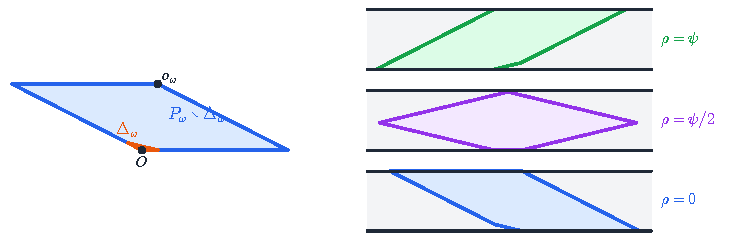
\includegraphics[width=\linewidth]{figures/fig-rotate}
\caption{\cref{lem:width,lem:turn}, for $\omega=1.1$. Left: the parallelogram $P_\omega$ (dashed), its corner triangle $\Delta_\omega$
(orange) and the pentagon $P_\omega\setminus\Delta_\omega$ (blue); the sofa $K\setminus\cN(K)$ lies in the pentagon, up to the far side of $\Delta_\omega$.
Right: the pentagon turned by $\rho=\psi$, $\psi/2$ and $0$, $\psi=\pi/2-\omega$, in a horizontal strip of width one: it fits for
every $\rho\in[0,\psi]$, since its width in the direction $u_t$ is at most $1$ for $t\in[\omega,\pi/2]$.}
\label{fig:rotate}
\end{figure}

\begin{proposition}[a right-angle monotone sofa]\label{prop:U}
Let $\omega\in[\omega_0,\pi/2]$ and let $T$ be a monotone sofa with rotation angle $\omega$, $\abs T=\abs\Gs$, and
cap $K=\cC(T)$, as in \cref{prop:reduction}. Then $R_\psi T$, $\psi=\pi/2-\omega$, is a moving sofa with rotation angle
$\pi/2$. Consequently there are $w_1\in\R^2$ and a monotone sofa $U$ with rotation angle $\pi/2$ such that
\[
  R_\psi T+w_1\subset U,\qquad\abs U=\abs\Gs,
\]
and the cap $\cC(U)\in\Kc_{\pi/2}$ is maximizing, with $\cA(\cC(U))=\abs\Gs$.
\end{proposition}

\begin{proof}
If $\omega=\pi/2$, $\psi=0$ and $T$ is a moving sofa with rotation angle $\pi/2$. Let $\omega<\pi/2$. The cap $K$ is
maximizing with $\cA_\omega(K)=\abs\Gs\ge11/5$, so \cref{prop:pinned-bounds} applies to $K_*=K$ and gives the pinned
bounds, \cref{lem:triangle} puts the vertices of $\Delta_\omega$ in some $Q^-_K(t_\sharp)$, and \cref{lem:width}(b) gives
$\ip{p-q}{u_t}\le1$ for $p,q\in T=K\setminus\cN(K)$ and $t\in[\omega,\pi/2]$. By \cref{lem:turn}, $R_\psi T$ is a moving
sofa with rotation angle $\pi/2$, and $\abs{R_\psi T}=\abs\Gs$. The second part is \cref{prop:reduction} for the
moving sofa $S'=R_\psi T$.
\end{proof}

By \cref{prop:reduction,prop:U}, there are $w_0,w_1\in\R^2$ such that, with $g_1(p)=R_\psi(p+w_0)+w_1$,
\begin{equation}\label{eq:contained}
  g_1(S)\subset U,\qquad \abs U=\abs\Gs,
\end{equation}
where $U$ is a monotone sofa with rotation angle $\pi/2$ whose cap is maximizing.
